\chapter[Referencial Teórico]{Referencial Teórico}

Neste capítulo, serão abordados conceitos que são imprescindíveis para a compreensão do trabalho em questão.

\section{Mercado de Moedas}

\subsection{Análise Técnica}
Existem dois tipos principais de análises no Mercado de Moedas, análise fundamental e análise técnica.

Análise fundamental é baseada no sentido de que acontecimentos mundiais tem impacto direto e são refletidos depois de algum tempo no mercado de moedas, assim sendo,
negociadores podem tirar proveito disso e trocar moedas baseando em por exemplo, notícias a respeito de algum país, entendendo o mercado
mundial como um todo e sabendo evidenciar os acontecimentos que terão algum impacto no Mercado de Moedas. Exemplos de notícias que afetam
o Mercado de Moedas são notícias a respeito de recursos.

Análise técnica é a análise em que este trabalho se baseia, e parte do pressuposto que toda a informação refletida no Mercado de Moedas está
contida no preços dos pares. Este tipo de análise se baseia principalmente na análise dos gráficos e indicadores, acreditando que se toda
informação está contida nos gráficos, não é necessário analisar notícias, acontecimentos e o calendário econômico por exemplo. Análise técnica
se encaixa mais neste estudo por ser mais precisa, enquanto a análise fundamental se baseia no próprio conhecimento do negociador, podendo muitas
vezes ser uma opinião subjetiva deste. A análise técnica busca evidenciar padrões e regras para tentar prever os movimentos do mercado.

\subsection{Tendência}

Analisando um gráfico do mercado de moedas, pode-ser observar algumas vezes claramente, outras não, o conceito de tendência que nada mais é
do que o sentido geral em que um par de negociação está se movimentando.

Na figura 01 consegue-se observar o sentido claramente, sabendo que o valor do par está aumentando em função do tempo.
Em alguns casos é mais difícil saber qual a tendência do mercado, como mostrado na figura 02.

\begin{figure}[h]
	\centering
	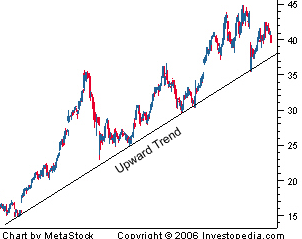
\includegraphics[keepaspectratio=true,scale=1]{figuras/up.png}
	\caption{Tendência de Subida}
	\label{fig01}
\end{figure}

\begin{figure}[h]
	\centering
	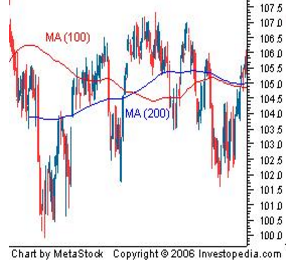
\includegraphics[keepaspectratio=true,scale=1]{figuras/flat.png}
	\caption{Tendência}
	\label{fig02}
\end{figure}


\subsection{Suporte}

Níveis de suporte são níveis que históricamente os preços tem dificuldade em cair abaixo, agindo assim como uma linha de suporte.

Na figura 03 pode-se perceber que ao longo do tempo, o preço da cotação apresentou certa resistência em ultrapassar o nível de suporte de 51.25

\begin{figure}[h]
	\centering
	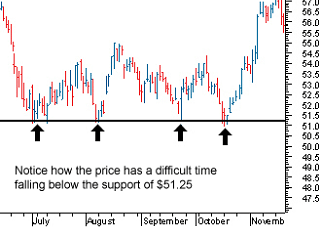
\includegraphics[keepaspectratio=true,scale=1]{figuras/sup.png}
	\caption{Suporte}
	\label{fig03}
\end{figure}

\subsection{Resistência}

Níveis de resistência são exatamente o contrário de níveis de suporte, representando valores aos quais o preço históricamente tem dificuldade
em ultrapassar acima. O momento em que uma cotação ultrapassa uma linha de resistência é frequentemente chamado de breakout.

\begin{figure}[h]
	\centering
	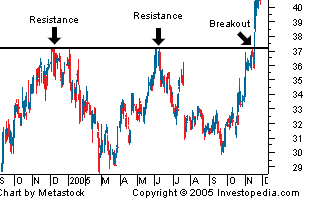
\includegraphics[keepaspectratio=true,scale=1]{figuras/resist.png}
	\caption{Resistência}
	\label{fig04}
\end{figure}

\subsection{Indicadores}

Para entender os indicadores utilizados no Mercado de Moedas, é preciso saber que os preços são mostrados divididos em quatro valores:
\begin{itemize}
  \item Low: Menor cotação da moeda
  \item Open: Valor de entrada de acordo com a janela de tempo escolhida
  \item Close: Valor de fechamento de acordo com a janela de tempo escolhida
  \item High: Maior cotação da moeda
\end{itemize}

A figura 05 mostra um exemplo de como esses valores são evidenciados num gráfico do Mercado de Moedas

\begin{figure}[h]
	\centering
	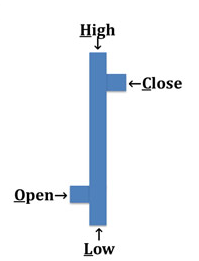
\includegraphics[keepaspectratio=true,scale=1]{figuras/price.png}
	\caption{Preço}
	\label{fig05}
\end{figure}



\section{Redes Neurais}

\subsection{Rede Neural Recorrente}
\subsection{LSTM}

\section{SCRUM}

\section{Teste de Software}
\subsection{Testes Unitários}
\subsection{Testes de Integração}
